\section{The FRG in LPA for the Gross-Neveu-Yukawa model}\label{sec:gny_frg}
\begin{disclaimer}
	This section follows the discussion presented in Secs. III and IV and App. G of \ccite{Stoll:2021ori}.
\end{disclaimer}
After the introduction of the \gnyBm{} on the level of the classical action, we will now focus on the application of the \frg{} to this model.
We will use the \frg{} to investigate the research questions outlined in the introduction.
The goals are to use the \frg{} to study the \gnyBm{} both at finite and infinite $N$.
Especially our study at finite $N$ will serve as the first application of our developments of \cref{chap:zeroONSU2} to higher-dimensional models.
This study will be focused on developing a detailed understanding of both fermionic and bosonic quantum and thermal fluctuations in our \cfd{} framework for the \frg{}.\bigskip

We have introduced the \frg{} on a formal level in \cref{sec:FRG} and we have discussed its application to zero-dimensional theories at length in the previous \cref{chap:zeroONSU2}. 
The major conceptual and practical challenge arising in \frg{} studies in non-zero dimensions is the fact that the \frgEq{} manifests as a functional differential equation which can not be solved directly.
As discussed in \cref{subsubsec:truncation}, truncations are necessary to project from the functional flow equation onto a finite set of \odes{} and/or \pdes{}.

We are aware that the \frg{} (at least in simple truncations like the \lpa{}) is usually not the method of choice for quantitative high precision predictions. 
But it has several advantages when it comes to the research questions addressed in this work. 
The \frg{} naturally resolves fluctuation effects \dash{} including fermionic and bosonic quantum and thermal fluctuations \dash{} at different energy scales and provides direct access to our observables of interest (the condensate, the curvature masses and the effective potential) at all scales $k ( t )$. 
The \frg{} as a continuum method can be used for direct computations in infinite volumes, incorporating quantum and thermal fluctuations non-perturbatively over a huge range of energies (wavelengths).
Computations in finite volumes are also possible within the \frg{} framework.
Actually, we plan to repeat the analysis of this work for the \gnym{} in a finite spatial volume along the lines of Refs.~\cite{Braun:2004yk,Braun:2005gy,Braun:2005fj,Braun:2011iz,Braun:2011uq} elsewhere, in order to directly analyze the effects of a finite sized spatial volume and to compare our results to the ones obtained with lattice Monte-Carlo simulations~\cite{Cohen:1981qz,Cohen:1983nr,Karsch:1986hm,Lenz:2020bxk,Lenz:2020cuv,Pannullo:2019bfn,Pannullo:2019prx}.
	
The advantages and shortcomings of our \frg{} setup for the \gnym{} will become clear within the following elaborations, where we introduce our truncation scheme and the explicit \frg{} flow equation.
We will comment on the limitations of our approach, and discuss symmetry restoration/breaking within the \frg{} approach.

\subsection{The GNY model in LPA truncation}\label{subsec:gnyLPA}
In the context of this work, we use the \acrrepeat{lpa}, introduced in \deRef{}, as a truncation for the \frgEq{}. 
For the \gnym{} this means that the \eaa{} is approximated as
\begin{align}
	\bar{\Gamma}_t [\varphi ,\psi, \bar{\psi}] = \, & \int \dif x\int_{0}^{\beta}  \dif \tau \, \big[ \bar{\psi} \, \big( \gamma^\nu\partial_\nu - \mu \gamma^2 + \tfrac{h}{\sqrt{N}} \, \varphi \big) \, \psi - \tfrac{1}{2} \, \varphi \, ( \Box \varphi ) + U ( t, \varphi ) \big] \ .	\label{eq:gnyLPAansatz}
\end{align}
In this ansatz exclusively the \rgscaledependent{} effective potential $U ( t, \varphi )$ is evolving with \rgtime{} $t$ (along \rgscale{} $k ( t )$), while all other couplings (\eg{}, the Yukawa coupling $h$) are kept constant.

Although being a rather simplistic ansatz, the \lpa{} is established as a common and powerful truncation scheme and is widely \dash{} arguably sometimes wildly --	used in the \frg{} community, especially in the context of strongly interacting systems, \eg{}, low-energy effective models, \cf{}\ \ccite{Dupuis:2020fhh} and references therein.
In the absence of fermions, the \lpa{} can be viewed as the lowest-order contribution of a derivative expansion, \cf{} \deRef{} and references therein.
The \lpa{} is assumed to be (and is for certain setups proven to be~\cite{DAttanasio:1997yph,Grossi:2019urj,Grossi:2021ksl,Koenigstein:2021syz,Koenigstein:2021rxj,Steil:2021cbu,Keitel:2011pn}) a good option for systems that are strongly coupled in field space and systems, where interactions with low-momentum transfer dominate the dynamics.
For further discussions on the quality or the comparison of truncation schemes, see, \cref{subsubsec:truncation} and in this context also \ccite{Balog:2019rrg,Eser:2018jqo,Eser:2019pvd,Divotgey:2019xea,Cichutek:2020bli}.
	
When dealing with the effects of long-range interactions (low momenta) in a low-dimensional model at non-zero $\mu$ and $T$ (strong coupling and complicated dynamics in field space), that we are heading at, the \lpa{} presents as a natural starting point for an analysis beyond the mean-field approximation.
We are aware, that the inclusion of scale-dependent and potentially even field-dependent wave-function renormalizations and couplings (especially a scale- and potentially field-dependent Yukawa coupling $h ( t, \varphi )$) would result in a significantly improved truncation. We will come back to this in \cref{paragraph:GNbGNGNY}.
For the moment we will just start off with the \lpa{}, which is already an improvement compared to the commonly used mean-field approximations for the \gnyBm{}, where the effects of bosonic quantum fluctuations are usually completely ignored or compared to ``improved'' mean-field approximations, see, \eg{}, \ccite{Dashen:1974xz}, which include only specific (effects of) bosonic modes{}.\bigskip
	
The \frg{} flow equation for the effective potential in the \lpa{} is obtained, by inserting the ansatz \eqref{eq:gnyLPAansatz} for $\bar{\Gamma}_t [\varphi, \psi, \bar{\psi}]$ into the \frgEq{} followed by a projection onto a suited (here constant) background field configuration
\begin{align}
	\FSsfEoM{}=\MFEchi{}\equiv (\MFEphi,\MFEpsi,\MFEpsib)=(\sigma,0,0)\, ,\label{eq:GNYVEV}
\end{align}
analogous to our discussion in \cref{subsubsec:0dSU2modelInt} of the zero-dimensional $SU(2)$ model, see also Chap. 23 of \ccite{Kleinert:2016}.
Additionally one has to specify proper, explicit regulators.
For a discussion on suitable choice and influences of different regulators on the \frg{} flow and the \ir{} results within a truncation, we refer to \ccite{Litim:2000ci,Litim:2001up,Pawlowski:2015mlf,Braun:2020bhy} and the discussion in the \customref{paragraph:comment_on_the_regulators}{next paragraph}.
In the context of our work, we use a one-dimensional \lpa{}-optimized momentum-space regulator for fermions and bosons~\cite{Litim:2000ci,Litim:2001up}, see \cref{subsubsec:regulator} for general remarks and \cref{app:GNvpr} for specifics.

Additionally and analogously to mean-field studies, we perform a rescaling of the bosonic (background) field and the scale-dependent effective potential,
\begin{subequations}\label{eq:rescaling_with_n}
\begin{align}
	\varphi \mapsto \, & \tilde{\varphi} = \tfrac{1}{\sqrt{N}} \, \varphi \, ,	\label{eq:rescaling_with_n_phi}
	\\
	U ( t, \varphi ) \mapsto \, & \tilde{U} ( t, \tilde{\varphi} ) = \tfrac{1}{N} \, U ( t, \varphi ) \, .\label{eq:rescaling_with_n_U}
\end{align}
\end{subequations}
This rescaling allows for a comparison of calculations at different finite values of $N$ and the infinite-$N$ limit.
In the following we are exclusively working in rescaled quantities $\tilde{\varphi}$ and $\tilde{U} ( t, \tilde{\varphi} )$, such that we do not maintain the ``tilde'' in our notation.
	
Using the propagators and regulator insertions of \cref{app:GNvpr}, we obtain the \lpa{} flow equation for the scale-dependent effective potential $U ( t, \sigma )$ in rescaled quantities, by performing all traces in field and internal spaces:
\begin{align}
	\partial_t U ( t,  \sigma ) &= \frac{1}{N} \, \Bigg(
	\frac{1}{2}\,\begin{gathered}
\includegraphics{gn/diagrams/GN2-UFlow2.pdf}\end{gathered}-\,\begin{gathered}
\includegraphics{gn/diagrams/GN2-UFlow1.pdf}\end{gathered}
	\Bigg)\\ 
	&= \, - \frac{1}{\piu N} \, \frac{k^3 ( t )}{2 E_{\textrm{b}} ( t, \partial^2_\sigma U )} \, \big[ 1 + 2 \, n_\mathrm{b} ( \beta E_{\textrm{b}} ( t, \partial^2_\sigma U ) ) \big] \,+ \notag\\*[.2em] % no page break
	& \qquad\qquad + \frac{d_\gamma}{\piu} \, \frac{k^3 ( t )}{2 E_{\textrm{f}}  ( t, \sigma )} \, \big[ 1 - n_\mathrm{f} ( \beta [ E_{\textrm{f}}  ( t, \sigma ) + \mu ] ) - n_\mathrm{f} ( \beta [ E_{\textrm{f}}  ( t, \sigma ) - \mu ] ) \big] \, ,		\label{eq:pdeq-U}
\end{align}
with $d_\gamma\equiv 2$, \cf{} \cref{app:spinors}, and where we introduced the abbreviations
\begin{subequations}
\begin{align}
	E_\mathrm{b} ( t, \partial^2_\sigma U ) \equiv \, & \sqrt{ k^2 ( t ) + \partial_\sigma^2 U ( t, \sigma ) } \, ,		\label{eq:Eb}
	\\[.2em]
	E_\mathrm{f} ( t, \sigma ) \equiv \, & \sqrt{ k^2 ( t ) + ( h \, \sigma )^2 } \, ,	\label{eq:Ef}
\end{align}
\end{subequations}
for the Euclidean bosonic and fermionic ``energies'' (dispersion relations) and used the distribution functions of \cref{app:matsubaraSums}.
Note that the prefactor $1/N$ of the bosonic contributions (the first term on the \rhs{} of \cref{eq:pdeq-U}) realizes the aforementioned suppression of bosonic fluctuations in the large-$N$ limit.
For the sake of completeness, all further details on the derivation of the flow equation are provided in \cref{app:GNlpa}.
Structurally this equation is (apart from the missing pionic contribution) reminiscent of the flow \cref{eq:SU2model0dUFlowExp} for the self-interaction potential of the zero-dimensional $SU(2)$ model.
We will comment on this further in \cref{subsec:lpaDSeq}.\bigskip
	
Before we continue our main discussion, we present the zero-temperature limit of the \frg{} flow equation \eqref{eq:pdeq-U},
\begin{align}
	\partial_t U ( t,  \sigma )	= \, & - \frac{1}{\piu N} \, \frac{k^3 ( t )}{2 E_\mathrm{b} ( t, \sigma )}  + \frac{d_\gamma}{\piu} \, \frac{k^3 ( t )}{2 E_\mathrm{f} ( t, \sigma )} \, \Theta \Big( 1 - \tfrac{\mu^2}{E^2_\mathrm{f} ( t, \sigma )} \Big)	\label{eq:zero_t_flow_equation}
\end{align}
as well as the vacuum limit for $T \rightarrow 0$ and $\mu \rightarrow 0$,
	\begin{align}
		\partial_t U ( t,  \sigma ) = \, & - \frac{1}{\piu N} \, \frac{k^3 ( t )}{2 E_\mathrm{b} ( t, \sigma )} + \frac{d_\gamma}{\piu} \, \frac{k^3 ( t )}{2 E_\mathrm{f} ( t, \sigma )} \, .	\label{eq:vacuum_limit_flow_equation}
	\end{align}
The \frg{} flow equation in vacuum is needed to fix the \ic{}.
	
Note that \cref{eq:vacuum_limit_flow_equation} differs from the popular \lpa{} flow equation of the effective potential for the $d=2$ \gnym{} in vacuum, \cf{}\ \ccite{Braun:2010tt,Rosa:2000ju},
\begin{align}
	\partial_t U ( t,  \sigma ) = \, & - \frac{1}{4 \piu N} \, \frac{k^4 ( t )}{2 E_\mathrm{b}^2 ( t, \sigma )} + \frac{d_\gamma}{4 \piu} \, \frac{k^4 ( t )}{2 E_\mathrm{f}^2 ( t, \sigma )} \, ,	\label{eq:2dim_litim_flow_equation}
\end{align}	
due to the fact that we are using one-dimensional purely spatial \lpa{}-optimized regulators in \cref{eq:vacuum_limit_flow_equation}.
Whereas \cref{eq:2dim_litim_flow_equation} is the flow equation for two-dimensional \lpa{}-optimized regulators.
We will comment on possible implications of this difference and the explicit breaking of Euclidean \Poincare{} invariance in the \customref{paragraph:comment_on_the_regulators}{next paragraph}, \cref{subsubsec:vacFiniteN_LD1} and \gnAppNum{}.

\paragraph{Comment on regulators}\phantomsection\label{paragraph:comment_on_the_regulators}\mbox{}\\%
At this point we ought to comment on the choice of our regulators and the caveats that go hand in hand with this choice.
The regulator shape functions \eqref{eq:gnregs} which parametrize the employed regulators, \cf{} \cref{eq:GNdtR}, only regulate the spatial momentum (direction).
Hence, if the spatial (loop) momenta are smaller than the \rgscale{} $k$, they are suppressed.
However, the Matsubara sums are not affected by the regulator at all and frequencies of all orders of magnitude enter the \frg{} flow at all scales $k ( t )$.
This has several direct consequences. 

Although regulators should in principle be in accordance with the symmetries of the theory, the employed regulators explicitly break (Euclidean) \Poincare{} invariance.
Hence, we cannot expect to recover full (Euclidean) \Poincare{} symmetry in the limits $\mu \rightarrow 0$ and $T \rightarrow 0$, without the introduction of counter-terms (Ward identities) to account for this discrepancy, \eg{}, Refs.~\cite{Braun:2017srn,Pawlowski:2017gxj} and \cref{subsec:renomMF}.
This means that the \ir{} results of the \frg{} flow equation \eqref{eq:vacuum_limit_flow_equation} do not necessarily coincide with \ir{} results of the vacuum \lpa{} flow equation \eqref{eq:2dim_litim_flow_equation} that can be derived with two-dimensional \lpa{} optimized regulators, if one uses exactly the same \uv{} \ic{}.
Whether or not these differences manifest in physical observables in vacuum or even medium, since computations at non-zero $T$ and $\mu$ usually use an \uv{} \ic{} fixated in vacuum, depends on the observable, model, and truncation under consideration, see, \eg{}, \ccite{Braun:2017srn,Pawlowski:2017gxj} and \cref{subsec:renomMF}.
Within the scope of this work we performed some test comparing results obtained with a two-dimensional \lpa{}-optimized regulator to results obtained using the one-dimensional \lpa{}-optimized regulator in vacuum using identical \ics{}.
For a brief discussion see \gnAppVacFlow{}.
The situation for the \gnyBm{} might be discussed elsewhere in more detail especially regarding regulator-dependencies at non-zero temperature~\cite{Zorbach:2021thesis}.\bigskip
	
One might ask now, why we are \dash{} regardless of these facts \dash{} using one-dimensional \lpa{}-optimized regulators? The answer to this question has several aspects:
	
A first drawback of using two-dimensional regulators is that large classes of those regulators cause problems in the presence of chemical potentials and violate the so-called \textit{Silver-Blaze} property~\cite{Cohen:2003kd,Marko:2014hea,Khan:2015puu,Leonhardt:2019mpy}.
However, we are especially interested in calculations at non-zero $\mu$.
Coping with this challenge is part of state of the art research, see, \eg{}, \ccite{Braun:2017srn,Braun:2018bik,Braun:2020bhy}, and we do not want to enter this discussion within this work.
	
Secondly, the analytic evaluation of the Matsubara sums or the loop-momentum integrals in \cref{eq:flow_equation_after_traces} might become impossible or at least extremely challenging, which drastically complicates numerical computations.
The presence of numerical sums and integrals in the flow equation would significantly increase computation time and hinder an in-depth discussion at variable $T$, $\mu$ and $N$. 
	
Note that for non-zero temperature and chemical potential (Euclidean) \Poincare{} invariance is broken anyhow, such that explicitly breaking this symmetry via the regulators might not spoil the results too drastically.

Mainly to facilitate, speed up numerical computations, and to avoid any conceptual issues at $\mu > 0$ we decided to use one-dimensional, spatial Litim regulators within this work as a first significant step beyond mean-field computations.
	
Interestingly, the approach of exclusively regulating spatial momenta is similar to the common strategy employed in conventional mean-field studies at non-zero temperature including the mean-field computations for the \gnyBm{}~\cite{Dolan:1973qd,Harrington:1974tf,Jacobs:1974ys,Dashen:1974xz,Dashen:1975xh,Wolff:1985av}.
There Matsubara summations are usually executed analytically before momentum integrals are regulated at all.
Divergent contributions (usually associated with vacuum quantum fluctuations) to expressions are separated from convergent (usually thermal) contributions and only the divergent parts are regulated.
Both approaches include all thermal/Matsubara modes independent of \rgscale{}  or in case of mean-field studies of the chosen regularization scheme.
	
\paragraph{Truncations and \ics{} \dash{} Differences and similarities of \gn{}, \bgn{} and \gny{} models}\phantomsection\label{paragraph:GNbGNGNY}\mbox{}\\%
In \cref{sec:gny} we introduced three distinct models by specifying their actions: the \gnm{} defined by $S_\mathrm{GN}$ in \cref{eq:gn-model}, the \bgnm{} defined by $S_\mathrm{bGN}$ in \cref{eq:bgn-model} and ultimately the \gnym{} defined by $S$ in \cref{eq:gny-model}. 
In this paragraph we will elaborate on their differences and similarities in the \frg{} framework with special focus on the, in this context, central issues of truncations and \ics{} for their respective \eaas{} $\bar{\Gamma}_t [\varphi, \psi, \bar{\psi}]$.
As for all \frg{} flows (and \pdes{} in general) their respective solutions depend on the corresponding initial and possible \bc{}(s).
We discuss the (numerical) \bcs{} in field space at length in \cref{subsec:boundary_conditions_finite_volume} and solely focus on the \ic{} for the moment.

The \gnm{} and its bosonized version \dash{} the \bgnm{} \dash{} have an identical partition function and are thus physically equivalent.
The bosonization procedure/\hsTrafo{} is merely a technical reformulation with the goal to eliminate the four-Fermi coupling term $\propto ( \Fpsib \Fpsi )^2$ of the \gnm{} by introducing the auxiliary field $\phi$  with a mass term $\propto \phi^2$ and a Yukawa-Coupling term $\propto \phi \, \Fpsib \Fpsi$.
This reformulation facilitates computations especially for non-vanishing condensates $\varphi\equiv \langle \phi \rangle \propto \langle \Fpsib \Fpsi \rangle$, as discussed in the context of dynamical hadronization in composite \frg{} flows for \qcd{} in \cref{paragraph:qcdDynHad}.
The \ic{} for $\bar{\Gamma}_t [ \chi ]$ for the \frgEq{} is the classical action $S[ \chi ]$.
Within the \lpa{} truncation the only scale-dependent quantity is the potential $U ( t, \sigma )$ for which an appropriate \ic{} at $k ( t = 0) = \Lambda$ can be read off directly from the classical action,
\begin{align}
	U ( 0, \sigma ) = \, & \tfrac{h^2}{2 g^2} \, \sigma^2 \, ,	\label{eq:uv-initial}
\end{align}
while the Yukawa coupling $h$ keeps its initial value throughout the \frg{} flow in the \lpa{}.
Note that the two rescalings in \cref{eq:rescaling_with_n} cancel for the rescaled initial potential \eqref{eq:uv-initial}.
This \ic{} $U ( 0, \sigma )$ is valid both for the \bgn{} and \gnym{} and will be discussed further in \cref{subsec:UUV}.
	
The only difference between the \bgn{} (and by proxy the \gn{}) model and the \gnym{} is the kinetic term $-\phi \, ( \Box \phi )$ in the latter.
A corresponding contribution $- \varphi \, ( \Box \varphi )$ (in terms of classical/mean-fields $\varphi = \langle \phi \rangle$) is of course also present in the \lpa{} ansatz \eqref{eq:gnyLPAansatz} for $\bar{\Gamma}_t [\varphi, \psi, \bar{\psi}]$ of the \gnym{} to establish the proper \ic{} $\bar{\Gamma}_{t = 0} = S$.
Such a kinetic term is needed in the \frg{} framework to study the effect of bosonic quantum fluctuations of $\phi$ at finite $N$.
In consequence, the \lpa{} to the \gnym{} for $\bar{\Gamma}_t [\varphi, \psi, \bar{\psi}]$ seems incapable of resembling the \bgnm{} (\gnm{} by proxy) in the \uv{}.
One might argue that the results, which are obtained from the \frg{} flow equation \eqref{eq:pdeq-U} with \ic{} \eqref{eq:uv-initial}, are consequently not directly transferable to the \gnm{}.
It seems, as if bosonic quantum fluctuations, which are linked to the kinetic term, are artificially enhanced already at the beginning of the \frg{} flow, while they should actually be strongly suppressed (strictly speaking vanishing directly in the \uv{} when considering the limit $\Lambda\rightarrow\infty$) in the \bgnm{} \eqref{eq:bgn-model}, which starts without the kinetic term in the \uv{} and generates the term and bosonic fluctuations dynamically during the \frg{} flow.
	
From the \frg{} perspective, the intuitive way to cure this problem is the introduction of a bosonic wave-function renormalization in the kinetic term,
\begin{align}
	- \varphi \, ( \Box \varphi ) \rightarrow - Z_{\varphi} ( t ) \, \varphi \, ( \Box \varphi ) \, ,
\end{align}
and initializing ${1 \ggg Z_{\varphi} ( 0 )>0}$ in the \uv{} to make direct contact with the action \eqref{eq:bgn-model} of the \bgnm{}.
Initializing $Z_{\varphi} ( 0 )$ at exactly zero in the \uv{} would lead to complications in practical computation since, \eg{}, the renormalized mass term $\tfrac{1}{Z_\varphi ( t )} \, \partial_\sigma^2 U ( t, \sigma )$ in the dispersion relation \eqref{eq:Eb} would diverge. Besides technical problems $Z_{\varphi} ( 0 )=0$ at a finite \uv{} initial scale $\Lambda$ would also weakly violate \rg{}-consistency, \cf{} \cref{subsec:RGflow}, since fluctuations (especially fermionic ones) at scales $k>\Lambda$ would have already generated a small wave-function renormalization.
Initializing the wave-function renormalization with ${1 \ggg Z_{\varphi} ( 0 )>0}$ in the \uv{} at a sufficiently large \uv{} initial scale $\Lambda$ \dash{} large enough  at the initial scale and in doing so realizing \rgcy{} \dash{} leads to a direct suppression of bosonic fluctuations at the beginning of the \frg{} flow.
This is directly seen on the level of $\bar{\Gamma}_t [\varphi, \psi,\bar{\psi}]$, where the bosonic kinetic term is suppressed by its small prefactor $Z_\varphi ( t = 0 )$ in the \uv{}.
During the \frg{} flow $Z_\varphi ( t )$ will turn non-zero already by its fermionic loop contribution, \cf{}\ \ccite{Braun:2010tt,Braun:2011pp} and especially the corresponding discussion in \cref{subsec:stability}.
	
Hence, we already conclude at this point that a natural generalization of the \lpa{} truncation in this work is the inclusion of a bosonic wave-function renormalization, such that the \uv{} \ic{} for $\bar{\Gamma}_t [ \varphi, \psi,\bar{\psi}]$ in the \gnym{} really resembles the \bgn{} and \gnm{}.
First steps of such a generalization/improvement are discussed in \ccite{Koenigstein:2023wso}.

Finally, we have to briefly comment on another issue, which also stems from the truncation scheme and the mismatch of the \ics{} for the \bgn{} and \gny{} models. The original \gn{} action \eqref{eq:gn-model} as well as its bosonized counterpart in \cref{eq:bgn-model} without the kinetic term $-\phi \, ( \Box \phi )$ have only a single coupling constant $g^2$. The artificial Yukawa coupling $h$ introduced during the bosonization procedure can actually be absorbed in the bosonic field. In mean-field calculations, see below, this is evident, because all observables can be fixed via a single dimensionful parameter (\eg{}, the \ir{} bosonic curvature mass, the \ir{} fermion mass, the critical temperature \etc{}) for $\Lambda \rightarrow \infty$ and can be mapped into each other, if different renormalization schemes were chosen. Including bosonic fluctuations, \ie{}\ the kinetic term for the bosons, the Yukawa coupling $h$ can no longer be completely absorbed via appropriate substitutions. Hence, the model involves an additional parameter that needs to be fixed via some renormalization condition~\cite{ZinnJustin:2002ru} \dash{} even if we stick to quadratic initial potentials \eqref{eq:uv-initial}.

We will comment on our specific choice of initial condition and implications on the suppression of bosonic fluctuations in the \uv{} in \cref{subsec:UUV} after our discussions at infinite-$N$.

\paragraph{Dynamical symmetry breaking in FRG flows}\phantomsection\label{paragraph:GNdSB}\mbox{}\\%
Since the \frg{} is formulated in terms of the effective (average) action, we set the following criteria for (spontaneous) symmetry breaking.
	
The vacuum/ground state of a \qft{} is defined as the field configuration with least energy, which has to be a field configuration that minimizes the \ir{} effective action $\Gamma [ \chi ]$, \cf{}\ \ccite{Wetterich:2001kra,Weinberg:1996kr}.
Hence it has to be a solution to the \qeom{} \eqref{eq:QEOM} for the mean-fields $\chi\equiv (\varphi,\psi,\bar{\psi})$,
\begin{subequations}
\begin{align}
	0 \overset{!}{=} \frac{\delta \Gamma [\MFchi]}{\delta \MFphi}\bigg|_{\MFchi=\MFchi_\eom=\MFEchi} \, ,\\
	0 \overset{!}{=} \frac{\delta \Gamma [\MFchi]}{\delta \MFpsi}\bigg|_{\MFchi=\MFchi_\eom=\MFEchi}\, ,\\
	0 \overset{!}{=} \frac{\delta \Gamma [\MFchi]}{\delta \MFpsib}\bigg|_{\MFchi=\MFchi_\eom=\MFEchi} \, ,
\end{align}
\end{subequations}
Within our truncation \eqref{eq:gnyLPAansatz}, these equations reduce to the following three \pdes{}
\begin{subequations}
\begin{align}
	0 = \, & \Box \, \MFEphi  - \partial_\varphi U ( t_\mathrm{IR}, \MFEphi ) - \tfrac{h}{N} \, \MFEpsib\mkern2mu\MFEpsi \, .\label{eq:qeqom1}\\[.1em]
	0 = \, & ( \gamma^\nu\partial_\nu - \mu \gamma^2 + h \, \MFEphi ) \, \MFEpsi \, ,	\label{eq:qeqom2}\\[.1em]
	0 = \, & (\partial_\nu \MFEpsib) \gamma^\nu + \MFEpsib\,( \mu \gamma^2 - h \, \MFEphi ) \, ,	\label{eq:qeqom3}
\end{align}
\end{subequations}
Given their nature as \gmv{}, fermionic fields it is natural to consider the trivial solutions $\MFEpsi (x,\tau) = 0$ and $\MFEpsib (x,\tau) = 0$. 
In this chapter we do not consider explicit inhomogeneous condensation and hence assume $\MFEphi (x,\tau) = \mathrm{const}.\equiv\sigma$ such that \cref{eq:qeqom1} simply reduces to
\begin{align}
	0 \overset{!}{=} \partial_\sigma U ( t_\mathrm{IR}, \sigma ) \, .
\end{align}
In order to ensure that this extremum condition defines a minimum and not a maximum, we need the additional sufficient condition $\partial_\sigma^2 U ( t_\mathrm{IR}, \sigma ) > 0$ at the extremum, \viz{} a positive \ir{} curvature mass for $\sigma$.

Consequently, in the \frg{} framework a minimum $\sigma_\mathrm{min}$ of the scale-dependent effective potential $U ( t, \sigma )$ in the \ir{} (for $t \rightarrow \infty$) is considered to be a (translational invariant) ground state of our system.
The system is said to be in the symmetry broken phase, if $\sigma_\mathrm{min} \neq 0$, and in the symmetric phase if $\sigma_\mathrm{min} = 0$, because non-trivial $\sigma_\mathrm{min}$ break the \ZII{} symmetry of the vacuum as discussed in \cref{paragraph:gnyVac}.

\subsection{LPA flow equation as non-linear diffusion-source/sink equation}\label{subsec:lpaDSeq}
In this subsection we discuss the numerical implementation and manifestation in a \cfd{} context of the \lpa{} flow \cref{eq:pdeq-U} of the \gnym{}.
We already noted a striking resemblance between the \lpa{} flow \cref{eq:pdeq-U} of the \gnym{} in \dtwo{} and the flow \cref{eq:SU2model0dUFlowExp} of the $SU(2)$ model in \dzero{}.\
In this regard the bosonic contributions in \cref{eq:pdeq-U} are structurally similar to the ones encountered in the flow \cref{eq:WetterichEq0d,eq:o(1)_wetterich_equation} for the zero-dimensional $O(1)$/\ZII{} model.
Informed by our studies in \dzero{} of \cref{chap:zeroONSU2} we take a derivative \wrt{} $\sigma$ to arrive at a conservative form for the flow equation of $\partial_t\partial_\sigma U(t,\sigma)\equiv \partial_t u(t,\sigma)$:
\begin{align}
	\partial_t u(t,\sigma) = \dod{}{\sigma} Q ( t, \partial_\sigma u ) + S ( t, \sigma ) \, ,	\label{eq:pdeq-u}
\end{align}
where we introduced the non-linear diffusion flux
\begin{align}
	Q ( t, \partial_\sigma u ) &\equiv \,  - \frac{1}{\piu N} \, \frac{k^3 ( t )}{2 E_{\textrm{b}} ( t, \partial_\sigma u )} \, \big[ 1 + 2 \, n_\mathrm{b} ( \beta E_{\textrm{b}} ( t, \partial_\sigma u ) ) \big] \, ,		\label{eq:diffusion_flux}
\end{align}
and the non-linear source/sink term
\begin{align}
	 S ( t, \sigma ) &\equiv \, \dod{}{\sigma}\! \bigg( \frac{d_\gamma}{\piu} \, \frac{k^3 ( t )}{2 E_{\textrm{f}} ( t, \sigma )} \, \big[ 1 - n_\mathrm{f} ( \beta [ E_{\textrm{f}} ( t, \sigma ) + \mu ] ) - n_\mathrm{f} ( \beta [ E_{\textrm{f}} ( t, \sigma ) - \mu ] ) \big] \bigg) \, .\label{eq:source_sink}
\end{align}
In primitive form the parabolic diffusive contribution in \cref{eq:pdeq-u} reads
\begin{align}
	\dod{}{\sigma} Q ( t, \partial_\sigma u ) = \alpha ( t, \partial_\sigma u ) \, \partial_\sigma^2 u ( t, \sigma ) \, ,	\label{eq:heat_equation_analogy}
\end{align}

We have arrived at a non-linear heat equation with a complicated source term. 
This formulation allows for a direct application of our \cfd{} framework of \cref{chap:zeroONSU2,sec:conservationLaws}.
We have discussed diffusive contributions of the kind of \cref{eq:diffusion_flux} at length in \cref{subsec:0dO1Entropy} and in our methodological introduction of diffusion equations in \cref{subsec:hydroDiffusion}.
It turns out that we can apply the numerical tools and the \cfd{} framework developed in \dzero{} directly to the \lpa{} flow equation in \dtwo{}.
Therefore we completely refrain from commenting on boundary conditions, spatial discretization, and a discussion of numerical entropy at this point since we have already discussed those aspects at length in \cref{subsubsec:conservative_form,subsec:boundary_conditions_finite_volume,subsec:0dO1Entropy}.
The only novel aspect, compared to the numerical studies in \cref{sec:0dON}, is the interesting source/sink term \eqref{eq:source_sink} on which we will comment in the next paragraph.

\paragraph{Fermionic (thermodynamic) fluctuations as sinks and sources}\phantomsection\label{paragraph:chemical_potential_shock_wave}\mbox{}\\%
Formulating the \frg{} flow equation on the level of the derivative of the scale-dependent effective potential $u ( t,  \sigma ) = \partial_\sigma U ( t, \sigma )$ allows for a refined understanding of the dynamics induced by a non-vanishing chemical potential $\mu$ and fermionic fluctuations in general.
The interpretation of the purely fermionic contribution $S ( t, \sigma )$ in terms of a time-dependent source/sink term emerges naturally in the \cfd{} framework.
From \cref{eq:source_sink} we find that the ``fluid'' $u( t, \sigma )$ does not explicitly enter $S ( t, \sigma )$ and the contribution to the flow of $u( t, \sigma )$ solely depends on the time $t$ and position in the spatial direction $\sigma$.
Actually it presents on a formal level in our flow equation as a classical potential (similar to a Newtonian gravitational potential) of a conservative (external) force field acting on the fluid, \cf{}\ \cref{subsec:hydroSource} and \ccite{KTO2-0}.
Executing the $\sigma$-derivative in \cref{eq:source_sink} one finds that the term enters the flow equation \eqref{eq:pdeq-u} for $u( t, \sigma )$ with negative sign for $\mu=0$, which explains the denotation as a ``sink'' for $\sigma > 0$ and ``source'' for $\sigma < 0$ and is responsible for symmetry breaking during the flow at $\mu = 0$.
Note that the dynamics of $u ( t, \sigma )$ is antisymmetric in $\sigma$.
Due to this antisymmetry and \wlogA{}, we focus our discussion on $\sigma \in [ 0, \infty )$, where the ``sink'' interpretation is more natural. For negative $\sigma$ the dynamics has of course opposite sign.
The bosonic contributions in terms of non-linear diffusion tend to fill the ``sink'' or distribute the ``source'' that is caused by the fermions and work against symmetry breaking.
At non-zero $\mu$ the sink/source term \eqref{eq:source_sink} is not always manifest negative/positive: it has a rather intricate dynamic (especially at low and zero temperature) and manifests as either source or sink depending on the value for $\sigma$ at a given $\mu$ and $t$ for both \dash{} negative and positive $\sigma$.
We will spend the rest of this paragraph illuminating this interesting manifestation of chemical potential as externally induced shock waves/discontinuities in field space.
\customWidthFigure%
	[!t]%
	{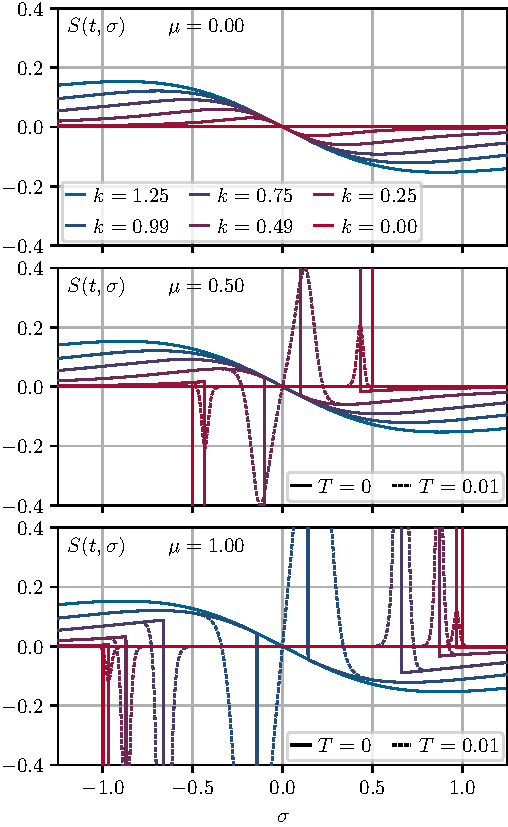
\includegraphics[width=7cm]{gn/figures/GN_sinkTerm.pdf}}% Graphics
	[]% Sublabels
	{%
		Source/sink term of \cref{eq:source_sink} at zero (solid lines) and small temperature $T=0.01$ (dashed lines) at various \rgscales{} $k$ (close to and below the model scales) between $k = 1.25$ in {blue} and $k = 0$ in {red} at $\mu = 0$ (upper panel), $\mu = 0.5$ (middle panel) and $\mu = 1.0$ (lower panel). All dimensionful quantities are measured in multiples of the Yukawa coupling $h$.
		\fromFig{1}{Stoll:2021ori}
	}%Caption
	{fig:GN_sinkTerm}%Label

It turns out that the chemical potential induces discontinuities in $u ( t, \sigma )$ in field space.
For the sake of simplicity, we analyze the \frg{} flow \cref{eq:pdeq-U} at vanishing (and small) temperature, \viz{} Eqs.~\eqref{eq:vacuum_limit_flow_equation} and~\eqref{eq:zero_t_flow_equation}, but on the level of $u ( t, \sigma )$, \cf{} \cref{eq:pdeq-u}.
We find that the difference between the $T = 0$ flow equations for $u ( t, \sigma )$ at vanishing and non-vanishing chemical potential is the contributions stemming from the derivative of the Heaviside function $\Theta ( 1 - \mu^2/E_\mathrm{f}^2 ( t, \sigma ) )$ in the source/sink term.
The sink/source term at different \rgscales{} and chemical potentials is plotted in \cref{fig:GN_sinkTerm} for $T=0$ and also small $T=0.01$ to support and illustrate the following discussion.
The approximate signs in the rest of this subsection hold at small temperatures and become exact for $T=0$.
	
As long as $E^2_\mathrm{f} \smallergtrsim \mu^2$, effects due the chemical potential do not manifest in the \frg{} flow, because $\mu$ does not show up in the source/sink term, see \cref{fig:GN_sinkTerm}.
However, when $E_\mathrm{f}^2 \approx \mu^2$, the chemical potential becomes relevant and distinguishes \frg{} flows with $\mu = 0$ and $\mu \neq 0$.
Therefore, it is important to understand when (in terms of \rgtime{} $t$), where (in field space $\sigma$), and how this is going to happen.
This can be done by analyzing the estimate
\begin{align}
	E_\mathrm{f}^2 = k^2 + ( h \sigma )^2 \approx \mu^2	\label{eq:influence_of_mu}
\end{align}
for different positions in field space.
	
The first time during the \frg{} flow, at which $\mu$ is going to influence the dynamics is, when $k^2 ( t ) \approx \mu^2$, \cf{} \cref{fig:GN_sinkTerm} at $k=0.99$ and $k=0.49$ in the middle and lower panel.
At this \rgscale{}, we find that the chemical potential will influence the dynamics at positions in field space close to $\sigma = 0$.
At slightly later \rgtimes{}, when $t$ is larger and the \rgscale{} $k ( t )$ is lowered a little, also field space positions at slightly larger $| \sigma |$ will be influenced by $\mu$.
The largest $| \sigma |$ that are directly affected by $\mu$ in the \pde{} are of the order $h^2 \sigma^2 \approx \mu^2$.
This is the case when $t \rightarrow \infty$ and $k ( t ) \rightarrow 0$ in \cref{eq:influence_of_mu}, \cf{} \cref{fig:GN_sinkTerm} at $k=0.0$ in the middle and lower panel.
The peaks induced by the chemical potential are located at ${\sigma\approx\pm \tfrac{1}{h}\sqrt{\mu^2-k(t)^2}}$ for $\mu \smallergtrsim k(t)$ and change the character of the sink/source term around their respective position.
For $\sigma>0$ ($\sigma<0$) the peak presents as a source (sink).
	 
Of course, the diffusive character of the $\sigma$-loop contribution will transport the effects of and the information about the chemical potential via diffusion also to larger $| \sigma |$.
The same holds true for the non-zero temperature version of the \frg{} flow \cref{eq:pdeq-u}, where the Heaviside function is smeared out in terms of a Fermi-Dirac distribution function \eqref{eq:nfDef}.
However, overall the \rgtime{} $t$ and scale $k ( t )$ as well as the relevant positions in field space $\sigma$ for the dynamics induced by the chemical potential are very similar at low temperatures where the dynamics is dominated by the chemical potential, \cf{} \cref{fig:GN_sinkTerm} for $T=0.01$.
	
The remaining question, that needs to be answered is, how the chemical potential $\mu$ \dash{} through the source term $S(t,\sigma)$ \dash{} influences the dynamics of the \frg{} flow.
We have argued before, that the fermionic contributions to the \frg{} flow of $u ( t, \sigma )$ enter as local time-dependent sink terms.
Now we found that the ``sinking'' stops suddenly at certain positions in field space and at certain \rgtimes{} during the \frg{} flow due to the chemical potential.
Hence, we expect that the chemical potential introduces a sharp edge in $u ( t, \sigma )$ at $\sigma \approx 0$, when $k^2 ( t ) \approx \mu^2$.
This edge will ``move'' in field space like a shock wave towards larger $| \sigma |$ until it reaches $| \sigma | \approx | \mu/h |$, where it comes to a halt.
This dynamics is imprinted by the underlying dynamics of the sink/source term \eqref{eq:source_sink} visualized and discussed earlier.
	
As already said before, this discontinuity is smeared by the diffusion an washed out right from the beginning at non-zero temperatures.
However, its dynamics is clearly underlying all diffusive processes.
In order to visualize the drastic effects of this discontinuity, we plot and contrast mean-field \frg{} flows with \frg{} flows involving bosonic fluctuations in \cref{subsubsec:chemical_potential_mf_vs_with_bosons}.
In mean-field, only the fermions are active (the sink term), such that the induced shock wave is not subject to diffusive effects and thus clearly visible.\bigskip
	
In fact, it is the chemical potential that introduces a jump (mean-field) or cusp (finite $N$) discontinuity in $u ( t, \sigma )$, which seems to render practical calculations at zero temperature involving bosonic fluctuations of the \sigmaMode{} impossible:
The discontinuity in $u ( t, \sigma )$ corresponds to a large jump in the derivative $\partial_\sigma u ( t, \sigma )$ with negative sign.
However, this happens at rather small $k^2 ( t ) \approx \mu^2$, such that the bosonic energy function,
\begin{align}
	E_\mathrm{b}^2 ( t, \partial_\sigma u ( t, \sigma ) ) = k^2 ( t) + \partial_\sigma u ( t, \sigma ) \, ,
\end{align}
turns negative and one overshoots the pole of the bosonic propagator $\tfrac{1}{E_\mathrm{b}}$ in the \frg{} flow equations.
Preventing further numerical evolution towards the \ir{}.
	
When considering a model involving also Goldstone modes{}, which enter the \frg{} flow as advective contributions, \cf{} \cref{subsec:0dONresults,subsec:0dLargeN} and \ccite{Grossi:2019urj,Grossi:2021ksl,Koenigstein:2021syz,Steil:2021cbu}, the huge gradients introduced via the chemical potential induce a shock wave that propagates towards smaller $|\sigma|$.
	
A possible reason, why this subtle dynamics in field space was not discussed in detail in the past within \frg{} studies might be that it is hardly visible and understandable on the level of the scale-dependent effective potential $U ( t, \sigma )$ itself, because it is the integral of $u ( t, \sigma )$, where jumps might only show up as tiny cusps, \cf{} \cref{subsubsec:chemical_potential_mf_vs_with_bosons}.
Additionally, a lot of previous studies did not perform calculations at sufficiently low temperatures, where this effect is not completely washed out by the thermal distribution functions \eqref{eq:nfDef}.
At this point the underlying reason for and resolution of this practical problem are not clear to the author.
The disconnection between the fermionic sector and the dynamics of $u(t,\sigma)$ in \lpa{}, the regulator choice or the formulation\footnote{A formal classification and proper weak formulation of the \pdes{} \eqref{eq:pdeq-U} and \eqref{eq:pdeq-u} might be paramount to understand the nature of the arising discontinuities and weak/physical solutions in their presence.} of the flow equation could be possible reasons for this intricate problem.
Solving this problem is beyond the scope of the current work. 
Consequently, we claim that understanding and/or capturing this effect correctly will be one of the central challenges in \frg{} at non-zero $\mu$ within the next years \dash{} independent of the specific models.
For related discussions on these novel findings, we also refer to \ccite{Grossi:2021ksl,Ihssen:2022xkr,Ihssen:2023xlp}.

\paragraph{Numerical implementation within our CFD framework}\phantomsection\label{paragraph:GNYKTnum}\mbox{}\\%
In this paragraph we present the explicit numeric implementation of the \frg{} flow equation~\eqref{eq:pdeq-u}.
To this end we adapt our developed and tested methods from \cref{sec:conservationLaws,sec:0dON}.

To adequately capture highly non-linear diffusive effects as well as the position-dependent source/sink terms, we adapt our implementation of the \ktScheme{}.
We use the scheme in its semi-discrete from \eqref{eq:FVKTO2} and for this chapter without the advective numerical fluxes, since we do not have advective contributions in the flow \cref{eq:pdeq-u}.
Within this chapter, we use the time-stepper \textit{solve\_ivp} with the \textit{LSODA} option using an Adams/BDF method with automatic stiffness detection and switching from the \textit{SciPy~1.0} library~\cite{2020SciPy-NMeth}.
For further details, see \gnAppNum{}.
We also cross-checked selected results with the \WAM{} codebase~\cite{Steil:2023zeroD,Steil:2023zeroDN1,Steil:2023zeroDlargeN,Steil:2023PhDFVNB} of \cref{chap:zeroONSU2}.
	
The explicit discretization of \cref{eq:pdeq-u}, \ie{}, the diffusion flux \eqref{eq:diffusion_flux} and sink term \eqref{eq:source_sink} is as follows.
We consider a compact computational domain $[ 0, \sigma_\mathrm{max} ]$, with boundary conditions according to \cref{subsec:boundary_conditions_finite_volume}, subdivided into $n \in \Integers{}$ equally sized (finite) volume cells of size $\Delta \sigma$ centered at positions $\sigma_i$, $i = 0, 1, \ldots, n - 1$.
The zeroth volume cell is centered at ${\sigma = \sigma_0 = 0}$, while the last cell is centered at $\sigma_{n - 1} = \sigma_\mathrm{max}$.
Within a single volume cell $\sigma_i$, the cell average of the ``fluid'' $u ( t, \sigma)$ is denoted as $\bar{u}_i ( t )$.
The actual computation and scheme is entirely formulated via these cell averages as discussed in \cref{sec:conservationLaws,sec:0dON}.
For the explicit implementation of boundary conditions one ghost cell is required at each interval boundary when considering a problem involving solely diffusive contributions in the semi-discrete \kt{}-scheme.
The ghost cells are of size $\Delta \sigma$ and centered at $\sigma_{-1} = - \Delta \sigma$ and $\sigma_{n} = \sigma_\mathrm{max} + \Delta \sigma$.
As described in \cref{subsec:boundary_conditions_finite_volume} we use the antisymmetry of $u ( t, \sigma )$ as boundary condition to fix the cell averages of the zeroth cell and first ghost cell to $\bar{u}_0 ( t ) = 0$ and $\bar{u}_{-1} ( t ) = - \bar{u}_{1} ( t )$ for all times $t$ respectively.
For the ghost cell at $\sigma_n$ we use linear extrapolation, thus for the cell average $\bar{u}_{n} ( t ) = 2 \, \bar{u}_{n - 1} ( t ) - \bar{u}_{n - 2} ( t )$ for all $t$.
Additionally, we consider as usual the grid of cell interfaces, which are positioned at $\sigma_{i + \ttfrac{1}{2}} \equiv \sigma_i + \tfrac{\Delta \sigma}{2}$.
	
Within this setup, the semi-discrete scheme for the non-linear diffusion-sink equation \eqref{eq:pdeq-u} and the evolution of the cell averages $\bar{u}_i ( t )$ reads~\cite{KTO2-0}
\begin{align}
	\partial_t \bar{u}_i = \tfrac{1}{\Delta \sigma} \, \big( P_{i + \frac{1}{2}} - P_{i - \frac{1}{2}} \big) + S_i \, ,
\end{align}
with the sink/source term $S_i = S ( t, \sigma_i )$ from \cref{eq:source_sink} and the numerical diffusion flux \eqref{eq:kt_original_diffusion} for the parabolic \gnym{} diffusion term \eqref{eq:diffusion_flux}.\bigskip

We conclude this brief discussion of the numerical implementation of \cref{eq:pdeq-u} with a comment on different discretization schemes for the sink/source term \eqref{eq:source_sink}.\bigskip

We want to put forward two possible discretization schemes for the source/sink term.
To arrive at these schemes, we return to the initial idea of the finite volume discretization outlined in \cref{subsec:hydroFV}.
Consider the integral form \eqref{eq:FVintEq} of the flow equation \eqref{eq:pdeq-u} for the $i^\text{th}$ cell 
\begin{align}
 \int_{\sigma_i - \frac{\Delta \sigma}{2}}^{\sigma_i + \frac{\Delta \sigma}{2}} \dif \sigma \, \partial_t u ( t, \sigma ) = \, & \int_{\sigma_i - \frac{\Delta \sigma}{2}}^{\sigma_i + \frac{\Delta \sigma}{2}} \dif \sigma \, \big[ \dod{}{\sigma} Q ( t, \partial_\sigma u ) + S ( t, \sigma ) \big] \, .\label{eq:GNYfinite_volume_scheme}
\end{align}
Keeping the control volumes fixed, one identifies the integral on the \lhs{} with the $t$-derivative of the cell averages of the fluid $\partial_t \bar{u}_i ( t )$ times $\Delta \sigma$. 
The integral over the $\sigma$-derivative of the diffusion flux on the \rhs{} is approximated using the numerical diffusion flux of the \ktScheme{}, \cf{} \cref{paragraph:KTQS}.
For the integral over the source/sink term $S ( t, \sigma )$ we basically consider two options.
\begin{enumerate}
	\item	The first option is an approximation. One approximates the source/sink term with $S ( t, \sigma_i )$ at the cell center times the cell-volume $\Delta \sigma$. Omitting the diffusive contribution, the semi-discrete flow equation for the cell averages $\bar{u}_i ( t )$ reads,
		\begin{align}
			\partial_t \bar{u}_i ( t ) = S ( t, \sigma_i ) \, ,	\label{eq:source_sink_1}
		\end{align}
	where we divided by $\Delta \sigma$.
	
	\item	The second option, which is due to a special feature of our \frg{} flow equation, is, to make use of the fact that the source/sink term in the flow \cref{eq:pdeq-u} presents as a spatial derivative of some function $s ( t, \sigma )$, which solely depends on $t$ and $\sigma$,
		\begin{align}
			S ( t, \sigma ) = \dod{}{\sigma}  s ( t, \sigma ) \, .	\label{eq:source_2}
		\end{align}
	This means that the integral on the \rhs{} of \cref{eq:GNYfinite_volume_scheme} can be calculated exactly, by evaluating $s ( t, \sigma )$ on the cell surfaces $\sigma_{i + \ttfrac{1}{2}}$.
	This results in,
		\begin{align}
			\partial_t \bar{u}_i ( t ) = \tfrac{1}{\Delta \sigma} \, \big[ s \big( t, \sigma_{i + \frac{1}{2}} \big) - s \big( t, \sigma_{i - \frac{1}{2}} \big) \big] \, ,	\label{eq:source_sink_2}
		\end{align}
	where we again omitted the diffusion flux for the sake of the present discussion and divided by $\Delta \sigma$.
\end{enumerate}

At first sight, it seems better to use the second exact version.
However, during our calculations, we did not experience any differences in precision between both versions for $T \neq 0$, as long as $\Delta \sigma$ is not too large.
Nevertheless, concerning the runtime, the first version turned out preferable in practical computations.
Eventually, this might be related to the fact, that, ignoring bosonic fluctuations (no diffusion), the first version reduces exactly to the mean-field calculation for $u ( t, \sigma )$ at positions $\sigma_i$, which can be directly seen from \cref{eq:source_sink_1}, where the \pde{} reduces into decoupled differential equations at the $\sigma_i$.

Though, for $T = 0$ the analytic evaluation of the $\sigma$-derivative would produce Dirac-delta distributions through the derivative of the Heaviside function, see \cref{eq:zero_t_flow_equation}. Delta-peaks are extremely complicated to implement in a numerical setup, but they are important at $T=0$ and should not be disregarded.
We therefore suggest to use the second version \eqref{eq:source_sink_2} (although it can only be used for \frg{}-mean-field calculations at $T=0$ for $u ( t, \sigma )$, which do not suffer from the problems described in \cref{paragraph:chemical_potential_shock_wave} and eluded to earlier in this paragraph).
	
We believe that there is some need for further investigations on the best discretization schemes for such fermionic contributions, see also \ccite{Grossi:2021ksl,Ihssen:2022xkr,Ihssen:2023xlp}.